
% Default to the notebook output style

    


% Inherit from the specified cell style.




    
\documentclass{article}

    
    
    \usepackage{graphicx} % Used to insert images
    \usepackage{adjustbox} % Used to constrain images to a maximum size 
    \usepackage{color} % Allow colors to be defined
    \usepackage{enumerate} % Needed for markdown enumerations to work
    \usepackage{geometry} % Used to adjust the document margins
    \usepackage{amsmath} % Equations
    \usepackage{amssymb} % Equations
    \usepackage{eurosym} % defines \euro
    \usepackage[mathletters]{ucs} % Extended unicode (utf-8) support
    \usepackage[utf8x]{inputenc} % Allow utf-8 characters in the tex document
    \usepackage{fancyvrb} % verbatim replacement that allows latex
    \usepackage{grffile} % extends the file name processing of package graphics 
                         % to support a larger range 
    % The hyperref package gives us a pdf with properly built
    % internal navigation ('pdf bookmarks' for the table of contents,
    % internal cross-reference links, web links for URLs, etc.)
    \usepackage{hyperref}
    \usepackage{longtable} % longtable support required by pandoc >1.10
    \usepackage{booktabs}  % table support for pandoc > 1.12.2
    \usepackage{mathpazo}
    \usepackage[spanish]{babel}

    
    
    \definecolor{orange}{cmyk}{0,0.4,0.8,0.2}
    \definecolor{darkorange}{rgb}{.71,0.21,0.01}
    \definecolor{darkgreen}{rgb}{.12,.54,.11}
    \definecolor{myteal}{rgb}{.26, .44, .56}
    \definecolor{gray}{gray}{0.45}
    \definecolor{lightgray}{gray}{.95}
    \definecolor{mediumgray}{gray}{.8}
    \definecolor{inputbackground}{rgb}{.95, .95, .85}
    \definecolor{outputbackground}{rgb}{.95, .95, .95}
    \definecolor{traceback}{rgb}{1, .95, .95}
    % ansi colors
    \definecolor{red}{rgb}{.6,0,0}
    \definecolor{green}{rgb}{0,.65,0}
    \definecolor{brown}{rgb}{0.6,0.6,0}
    \definecolor{blue}{rgb}{0,.145,.698}
    \definecolor{purple}{rgb}{.698,.145,.698}
    \definecolor{cyan}{rgb}{0,.698,.698}
    \definecolor{lightgray}{gray}{0.5}
    
    % bright ansi colors
    \definecolor{darkgray}{gray}{0.25}
    \definecolor{lightred}{rgb}{1.0,0.39,0.28}
    \definecolor{lightgreen}{rgb}{0.48,0.99,0.0}
    \definecolor{lightblue}{rgb}{0.53,0.81,0.92}
    \definecolor{lightpurple}{rgb}{0.87,0.63,0.87}
    \definecolor{lightcyan}{rgb}{0.5,1.0,0.83}
    
    % commands and environments needed by pandoc snippets
    % extracted from the output of `pandoc -s`
    \DefineVerbatimEnvironment{Highlighting}{Verbatim}{commandchars=\\\{\}}
    % Add ',fontsize=\small' for more characters per line
    \newenvironment{Shaded}{}{}
    \newcommand{\KeywordTok}[1]{\textcolor[rgb]{0.00,0.44,0.13}{\textbf{{#1}}}}
    \newcommand{\DataTypeTok}[1]{\textcolor[rgb]{0.56,0.13,0.00}{{#1}}}
    \newcommand{\DecValTok}[1]{\textcolor[rgb]{0.25,0.63,0.44}{{#1}}}
    \newcommand{\BaseNTok}[1]{\textcolor[rgb]{0.25,0.63,0.44}{{#1}}}
    \newcommand{\FloatTok}[1]{\textcolor[rgb]{0.25,0.63,0.44}{{#1}}}
    \newcommand{\CharTok}[1]{\textcolor[rgb]{0.25,0.44,0.63}{{#1}}}
    \newcommand{\StringTok}[1]{\textcolor[rgb]{0.25,0.44,0.63}{{#1}}}
    \newcommand{\CommentTok}[1]{\textcolor[rgb]{0.38,0.63,0.69}{\textit{{#1}}}}
    \newcommand{\OtherTok}[1]{\textcolor[rgb]{0.00,0.44,0.13}{{#1}}}
    \newcommand{\AlertTok}[1]{\textcolor[rgb]{1.00,0.00,0.00}{\textbf{{#1}}}}
    \newcommand{\FunctionTok}[1]{\textcolor[rgb]{0.02,0.16,0.49}{{#1}}}
    \newcommand{\RegionMarkerTok}[1]{{#1}}
    \newcommand{\ErrorTok}[1]{\textcolor[rgb]{1.00,0.00,0.00}{\textbf{{#1}}}}
    \newcommand{\NormalTok}[1]{{#1}}
    
    % Define a nice break command that doesn't care if a line doesn't already
    % exist.
    \def\br{\hspace*{\fill} \\* }
    % Math Jax compatability definitions
    \def\gt{>}
    \def\lt{<}
    % Document parameters
    \title{Trabajo Final - Sistemas con retardo en la entrada}
    
    
    

    % Pygments definitions
    
\makeatletter
\def\PY@reset{\let\PY@it=\relax \let\PY@bf=\relax%
    \let\PY@ul=\relax \let\PY@tc=\relax%
    \let\PY@bc=\relax \let\PY@ff=\relax}
\def\PY@tok#1{\csname PY@tok@#1\endcsname}
\def\PY@toks#1+{\ifx\relax#1\empty\else%
    \PY@tok{#1}\expandafter\PY@toks\fi}
\def\PY@do#1{\PY@bc{\PY@tc{\PY@ul{%
    \PY@it{\PY@bf{\PY@ff{#1}}}}}}}
\def\PY#1#2{\PY@reset\PY@toks#1+\relax+\PY@do{#2}}

\expandafter\def\csname PY@tok@s1\endcsname{\def\PY@tc##1{\textcolor[rgb]{0.73,0.13,0.13}{##1}}}
\expandafter\def\csname PY@tok@m\endcsname{\def\PY@tc##1{\textcolor[rgb]{0.40,0.40,0.40}{##1}}}
\expandafter\def\csname PY@tok@mh\endcsname{\def\PY@tc##1{\textcolor[rgb]{0.40,0.40,0.40}{##1}}}
\expandafter\def\csname PY@tok@nv\endcsname{\def\PY@tc##1{\textcolor[rgb]{0.10,0.09,0.49}{##1}}}
\expandafter\def\csname PY@tok@o\endcsname{\def\PY@tc##1{\textcolor[rgb]{0.40,0.40,0.40}{##1}}}
\expandafter\def\csname PY@tok@gp\endcsname{\let\PY@bf=\textbf\def\PY@tc##1{\textcolor[rgb]{0.00,0.00,0.50}{##1}}}
\expandafter\def\csname PY@tok@gu\endcsname{\let\PY@bf=\textbf\def\PY@tc##1{\textcolor[rgb]{0.50,0.00,0.50}{##1}}}
\expandafter\def\csname PY@tok@ge\endcsname{\let\PY@it=\textit}
\expandafter\def\csname PY@tok@sb\endcsname{\def\PY@tc##1{\textcolor[rgb]{0.73,0.13,0.13}{##1}}}
\expandafter\def\csname PY@tok@nd\endcsname{\def\PY@tc##1{\textcolor[rgb]{0.67,0.13,1.00}{##1}}}
\expandafter\def\csname PY@tok@vc\endcsname{\def\PY@tc##1{\textcolor[rgb]{0.10,0.09,0.49}{##1}}}
\expandafter\def\csname PY@tok@sc\endcsname{\def\PY@tc##1{\textcolor[rgb]{0.73,0.13,0.13}{##1}}}
\expandafter\def\csname PY@tok@na\endcsname{\def\PY@tc##1{\textcolor[rgb]{0.49,0.56,0.16}{##1}}}
\expandafter\def\csname PY@tok@se\endcsname{\let\PY@bf=\textbf\def\PY@tc##1{\textcolor[rgb]{0.73,0.40,0.13}{##1}}}
\expandafter\def\csname PY@tok@sd\endcsname{\let\PY@it=\textit\def\PY@tc##1{\textcolor[rgb]{0.73,0.13,0.13}{##1}}}
\expandafter\def\csname PY@tok@nf\endcsname{\def\PY@tc##1{\textcolor[rgb]{0.00,0.00,1.00}{##1}}}
\expandafter\def\csname PY@tok@kr\endcsname{\let\PY@bf=\textbf\def\PY@tc##1{\textcolor[rgb]{0.00,0.50,0.00}{##1}}}
\expandafter\def\csname PY@tok@nl\endcsname{\def\PY@tc##1{\textcolor[rgb]{0.63,0.63,0.00}{##1}}}
\expandafter\def\csname PY@tok@cp\endcsname{\def\PY@tc##1{\textcolor[rgb]{0.74,0.48,0.00}{##1}}}
\expandafter\def\csname PY@tok@vg\endcsname{\def\PY@tc##1{\textcolor[rgb]{0.10,0.09,0.49}{##1}}}
\expandafter\def\csname PY@tok@c\endcsname{\let\PY@it=\textit\def\PY@tc##1{\textcolor[rgb]{0.25,0.50,0.50}{##1}}}
\expandafter\def\csname PY@tok@gr\endcsname{\def\PY@tc##1{\textcolor[rgb]{1.00,0.00,0.00}{##1}}}
\expandafter\def\csname PY@tok@mb\endcsname{\def\PY@tc##1{\textcolor[rgb]{0.40,0.40,0.40}{##1}}}
\expandafter\def\csname PY@tok@go\endcsname{\def\PY@tc##1{\textcolor[rgb]{0.53,0.53,0.53}{##1}}}
\expandafter\def\csname PY@tok@gt\endcsname{\def\PY@tc##1{\textcolor[rgb]{0.00,0.27,0.87}{##1}}}
\expandafter\def\csname PY@tok@err\endcsname{\def\PY@bc##1{\setlength{\fboxsep}{0pt}\fcolorbox[rgb]{1.00,0.00,0.00}{1,1,1}{\strut ##1}}}
\expandafter\def\csname PY@tok@mo\endcsname{\def\PY@tc##1{\textcolor[rgb]{0.40,0.40,0.40}{##1}}}
\expandafter\def\csname PY@tok@mf\endcsname{\def\PY@tc##1{\textcolor[rgb]{0.40,0.40,0.40}{##1}}}
\expandafter\def\csname PY@tok@gd\endcsname{\def\PY@tc##1{\textcolor[rgb]{0.63,0.00,0.00}{##1}}}
\expandafter\def\csname PY@tok@nc\endcsname{\let\PY@bf=\textbf\def\PY@tc##1{\textcolor[rgb]{0.00,0.00,1.00}{##1}}}
\expandafter\def\csname PY@tok@sr\endcsname{\def\PY@tc##1{\textcolor[rgb]{0.73,0.40,0.53}{##1}}}
\expandafter\def\csname PY@tok@k\endcsname{\let\PY@bf=\textbf\def\PY@tc##1{\textcolor[rgb]{0.00,0.50,0.00}{##1}}}
\expandafter\def\csname PY@tok@si\endcsname{\let\PY@bf=\textbf\def\PY@tc##1{\textcolor[rgb]{0.73,0.40,0.53}{##1}}}
\expandafter\def\csname PY@tok@ss\endcsname{\def\PY@tc##1{\textcolor[rgb]{0.10,0.09,0.49}{##1}}}
\expandafter\def\csname PY@tok@ow\endcsname{\let\PY@bf=\textbf\def\PY@tc##1{\textcolor[rgb]{0.67,0.13,1.00}{##1}}}
\expandafter\def\csname PY@tok@sx\endcsname{\def\PY@tc##1{\textcolor[rgb]{0.00,0.50,0.00}{##1}}}
\expandafter\def\csname PY@tok@vi\endcsname{\def\PY@tc##1{\textcolor[rgb]{0.10,0.09,0.49}{##1}}}
\expandafter\def\csname PY@tok@ne\endcsname{\let\PY@bf=\textbf\def\PY@tc##1{\textcolor[rgb]{0.82,0.25,0.23}{##1}}}
\expandafter\def\csname PY@tok@il\endcsname{\def\PY@tc##1{\textcolor[rgb]{0.40,0.40,0.40}{##1}}}
\expandafter\def\csname PY@tok@kt\endcsname{\def\PY@tc##1{\textcolor[rgb]{0.69,0.00,0.25}{##1}}}
\expandafter\def\csname PY@tok@nb\endcsname{\def\PY@tc##1{\textcolor[rgb]{0.00,0.50,0.00}{##1}}}
\expandafter\def\csname PY@tok@kp\endcsname{\def\PY@tc##1{\textcolor[rgb]{0.00,0.50,0.00}{##1}}}
\expandafter\def\csname PY@tok@kd\endcsname{\let\PY@bf=\textbf\def\PY@tc##1{\textcolor[rgb]{0.00,0.50,0.00}{##1}}}
\expandafter\def\csname PY@tok@s\endcsname{\def\PY@tc##1{\textcolor[rgb]{0.73,0.13,0.13}{##1}}}
\expandafter\def\csname PY@tok@kn\endcsname{\let\PY@bf=\textbf\def\PY@tc##1{\textcolor[rgb]{0.00,0.50,0.00}{##1}}}
\expandafter\def\csname PY@tok@cs\endcsname{\let\PY@it=\textit\def\PY@tc##1{\textcolor[rgb]{0.25,0.50,0.50}{##1}}}
\expandafter\def\csname PY@tok@no\endcsname{\def\PY@tc##1{\textcolor[rgb]{0.53,0.00,0.00}{##1}}}
\expandafter\def\csname PY@tok@nn\endcsname{\let\PY@bf=\textbf\def\PY@tc##1{\textcolor[rgb]{0.00,0.00,1.00}{##1}}}
\expandafter\def\csname PY@tok@bp\endcsname{\def\PY@tc##1{\textcolor[rgb]{0.00,0.50,0.00}{##1}}}
\expandafter\def\csname PY@tok@mi\endcsname{\def\PY@tc##1{\textcolor[rgb]{0.40,0.40,0.40}{##1}}}
\expandafter\def\csname PY@tok@gh\endcsname{\let\PY@bf=\textbf\def\PY@tc##1{\textcolor[rgb]{0.00,0.00,0.50}{##1}}}
\expandafter\def\csname PY@tok@nt\endcsname{\let\PY@bf=\textbf\def\PY@tc##1{\textcolor[rgb]{0.00,0.50,0.00}{##1}}}
\expandafter\def\csname PY@tok@gs\endcsname{\let\PY@bf=\textbf}
\expandafter\def\csname PY@tok@ni\endcsname{\let\PY@bf=\textbf\def\PY@tc##1{\textcolor[rgb]{0.60,0.60,0.60}{##1}}}
\expandafter\def\csname PY@tok@cm\endcsname{\let\PY@it=\textit\def\PY@tc##1{\textcolor[rgb]{0.25,0.50,0.50}{##1}}}
\expandafter\def\csname PY@tok@c1\endcsname{\let\PY@it=\textit\def\PY@tc##1{\textcolor[rgb]{0.25,0.50,0.50}{##1}}}
\expandafter\def\csname PY@tok@sh\endcsname{\def\PY@tc##1{\textcolor[rgb]{0.73,0.13,0.13}{##1}}}
\expandafter\def\csname PY@tok@s2\endcsname{\def\PY@tc##1{\textcolor[rgb]{0.73,0.13,0.13}{##1}}}
\expandafter\def\csname PY@tok@gi\endcsname{\def\PY@tc##1{\textcolor[rgb]{0.00,0.63,0.00}{##1}}}
\expandafter\def\csname PY@tok@w\endcsname{\def\PY@tc##1{\textcolor[rgb]{0.73,0.73,0.73}{##1}}}
\expandafter\def\csname PY@tok@kc\endcsname{\let\PY@bf=\textbf\def\PY@tc##1{\textcolor[rgb]{0.00,0.50,0.00}{##1}}}

\def\PYZbs{\char`\\}
\def\PYZus{\char`\_}
\def\PYZob{\char`\{}
\def\PYZcb{\char`\}}
\def\PYZca{\char`\^}
\def\PYZam{\char`\&}
\def\PYZlt{\char`\<}
\def\PYZgt{\char`\>}
\def\PYZsh{\char`\#}
\def\PYZpc{\char`\%}
\def\PYZdl{\char`\$}
\def\PYZhy{\char`\-}
\def\PYZsq{\char`\'}
\def\PYZdq{\char`\"}
\def\PYZti{\char`\~}
% for compatibility with earlier versions
\def\PYZat{@}
\def\PYZlb{[}
\def\PYZrb{]}
\makeatother


    % Exact colors from NB
    \definecolor{incolor}{rgb}{0.0, 0.0, 0.5}
    \definecolor{outcolor}{rgb}{0.545, 0.0, 0.0}



    
    % Prevent overflowing lines due to hard-to-break entities
    \sloppy 
    % Setup hyperref package
    \hypersetup{
      breaklinks=true,  % so long urls are correctly broken across lines
      colorlinks=true,
      urlcolor=blue,
      linkcolor=darkorange,
      citecolor=darkgreen,
      }
    % Slightly bigger margins than the latex defaults
    
    \geometry{verbose,tmargin=1in,bmargin=1in,lmargin=1in,rmargin=1in}
    
    \author{Roberto Cadena Vega}

    \begin{document}
    
    
    \maketitle

    
    
    \section{Recapitulación de resultados
empleados}\label{recapitulaciuxf3n-de-resultados-empleados}

    \subsection{Control predictivo}\label{control-predictivo}

    \subsection{Implementación del retardo distribuido y sus
problemas}\label{implementaciuxf3n-del-retardo-distribuido-y-sus-problemas}

    \subsection{Solución por medio de estabilización
simultanea}\label{soluciuxf3n-por-medio-de-estabilizaciuxf3n-simultanea}

    \subsection{Solución por medio de introducción de
dinámicas}\label{soluciuxf3n-por-medio-de-introducciuxf3n-de-dinuxe1micas}

    \section{Implementación de control predictivo: ejemplo
escalar}\label{implementaciuxf3n-de-control-predictivo-ejemplo-escalar}

    \subsection{\texorpdfstring{Resultados del articulo ``Some problems
arising in the implementation of distributed-delay control
laws''}{Resultados del articulo Some problems arising in the implementation of distributed-delay control laws}}\label{resultados-del-articulo-some-problems-arising-in-the-implementation-of-distributed-delay-control-laws}

    \section{Implementación del método de estabilización
simultanea}\label{implementaciuxf3n-del-muxe9todo-de-estabilizaciuxf3n-simultanea}

    \subsection{Ejemplo 1 - Doble integrador
retardado}\label{ejemplo-1---doble-integrador-retardado}

    Para el sistema:

\[
\dot{x}(t) =
\begin{pmatrix}
0 & 1 \\
0 & 0
\end{pmatrix}
x(t) +
\begin{pmatrix}
0 \\
1
\end{pmatrix}
u(t - h)
\]

con \(h = 1\).

    El cual, bajo una ley de control de la forma:

\[
u(t) = k \left[ x(t) + \int_{-h}^0 e^{-A(\theta + h)} B u(t + \theta) d\theta \right]
\]

tiene un polinomio caracteristico:

\[
s^2 +  \left( h k_1 - k_2 \right) s - k_1
\]

Al cual podemos aplicar el criterio de estabilidad de Routh-Hurwitz y
obtener:

\[
\begin{align}
k_1 &< 0 \\
k_2 &< h k_1
\end{align}
\]

Por lo que la gráfica de D-particiones del sistema en lazo cerrado se
verá:

\begin{figure}[htbp]
\centering
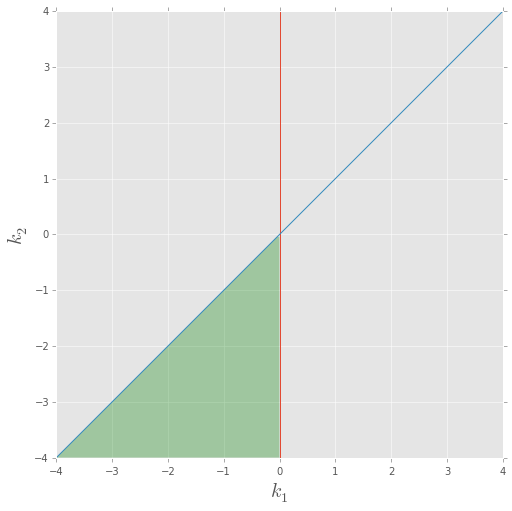
\includegraphics[width=0.5\textwidth]{../imagenes/dobintlc.png}
\caption{D-particiones de un doble integrador en lazo cerrado}
\end{figure}

    Por otro lado, para analizar el comportamiento del controlador,
sustituimos los datos en la ecuación del controlador:

\[
\begin{align}
u(t) &=
\begin{pmatrix}
k_1 & k_2
\end{pmatrix} x(t) +
\begin{pmatrix}
k_1 & k_2
\end{pmatrix}
\int_{-h}^0 e^{-A(\theta + h)} B u(t + \theta) d\theta \\
&=
\begin{pmatrix}
k_1 & k_2
\end{pmatrix}
\begin{pmatrix}
x_1(t) \\
x_2(t)
\end{pmatrix} +
\begin{pmatrix}
k_1 & k_2
\end{pmatrix}
\int_{-h}^0 e^{-A(\theta + h)} B u(t + \theta) d\theta \\
\end{align}
\]

    \[
\begin{align}
u(t) &=
\begin{pmatrix}
k_1 & k_2
\end{pmatrix}
\begin{pmatrix}
x_1(t) \\
x_2(t)
\end{pmatrix} +
\int_{-h}^0
\begin{pmatrix}
k_1 & k_2
\end{pmatrix}
\begin{pmatrix}
1 & - (\theta  +h) \\
0 & 1
\end{pmatrix}
\begin{pmatrix}
0 \\
1
\end{pmatrix} u(t + \theta) d\theta \\
&= k_1 x_1(t) + k_2 x_2(t) - \int_{-h}^0 k_1 \theta u(t + \theta) d\theta - \int_{-h}^0 k_1 h u(t + \theta) d\theta + \int_{-h}^0 k_2 u(t + \theta) d\theta \\
\end{align}
\]

y al aplicar la transformada de Laplace, tenemos:

\[
u(s) = k_1 x_1(s) + k_2 x_2(s) - h k_1 \frac{e^{-hs}}{s} u(s) + k_1 \frac{1 - e^{-hs}}{s^2} u(s) - h k_1 \frac{1 - e^{-hs}}{s} u(s) + k_2 \frac{1 - e^{-hs}}{s} u(s)
\]

por lo que al pasar a un solo lado todos los terminos de \(u(s)\):

\[
\begin{align}
\left[ 1 + h k_1 \frac{e^{-hs}}{s} - k_1 \frac{1 - e^{-hs}}{s^2} + h k_1 \frac{1 - e^{-hs}}{s} - k_2 \frac{1 - e^{-hs}}{s} \right] u(s) &= k_1 x_1(s) + k_2 x_2(s) \\
\left[ 1 + \frac{h k_1 e^{-hs}}{s} - \frac{k_1}{s^2} + \frac{k_1 e^{-hs}}{s^2} + \frac{h k_1}{s} - \frac{h k_1 e^{-hs}}{s} - \frac{k_2}{s} + \frac{k_2 e^{-hs}}{s} \right] u(s) &= k_1 x_1(s) + k_2 x_2(s) \\
\left[ 1  - \frac{k_1}{s^2} + \frac{k_1 e^{-hs}}{s^2} + \frac{h k_1}{s} - \frac{k_2}{s} + \frac{k_2 e^{-hs}}{s} \right] u(s) &= k_1 x_1(s) + k_2 x_2(s) \\
\left[ 1  + \frac{k_1 e^{-hs} - k_1}{s^2} + \frac{h k_1 + k_2 e^{-hs} - k_2}{s} \right] u(s) &= k_1 x_1(s) + k_2 x_2(s)
\end{align}
\]

obtenemos el polinomio caracteristico de la ecuación de control:

\[
1  + \frac{k_1 e^{-hs} - k_1}{s^2} + \frac{h k_1 + k_2 e^{-hs} - k_2}{s}
\]

y al sustituir \(s = j \omega\), obtendremos dos ecuaciones,
correspondientes a la parte real e imaginaria:

\[
\begin{align}
k_1 \left[ \omega h - \sin{(\omega h)} \right] - k_2 \left[ \omega - \cos{(\omega h)} \right] &= 0 \\
- k_1 \left[ 1 - \cos{(\omega h)} \right] + k_2 \left[ \omega \sin{(\omega h)} \right] - \omega^2 &= 0 \\
\end{align}
\]

por lo que podemos despejar \(k_2\) de ambas ecuaciones y obtener:

\[
k_2 = \frac{k_1 \left[ \omega h - \sin{(\omega h)} \right]}{\omega - \cos{(\omega h)}} = \frac{k_1 \left[ 1 - \cos{(\omega h)} \right] + \omega^2}{\omega \sin{(\omega h)}}
\]

y haciendo un poco de algebra, podemos obtener:

\[
\frac{k_1 \left[ \omega h - \sin{(\omega h)} \right]}{\omega - \cos{(\omega h)}} = \frac{k_1 \left[ 1 - \cos{(\omega h)} \right] + \omega^2}{\omega \sin{(\omega h)}}
\]

\[
\frac{k_1 \left[ \omega h - \sin{(\omega h)} \right] \left[ \omega \sin{(\omega h)} \right]}{\omega - \cos{(\omega h)}} - k_1 \left[ 1 - \cos{(\omega h)} \right] = \omega^2
\]

\[
k_1 \frac{\left[ \omega h - \sin{(\omega h)} \right] \left[ \omega \sin{(\omega h)} \right] - \left[ 1 - \cos{(\omega h)} \right] \left[ \omega - \cos{(\omega h)} \right]}{\omega - \cos{(\omega h)}} = \omega^2
\]

\[
k_1 = \frac{\omega^2 \left[ \omega - \cos{(\omega h)} \right]}{\left[ \omega h - \sin{(\omega h)} \right] \left[ \omega \sin{(\omega h)} \right] - \left[ 1 - \cos{(\omega h)} \right] \left[ \omega - \cos{(\omega h)} \right]}
\]

Si sustituimos un punto por debajo de esta curva,
\((k_1, k_2) = (0, 0)\), podemos ver que el polinomio caracteristico es
trivialmente estable por el criterio de Routh-Hurwitz:

\[
P(s) = 1
\]

por lo que la gráfica de D-particiones para el controlador queda:

\begin{figure}[htbp]
\centering
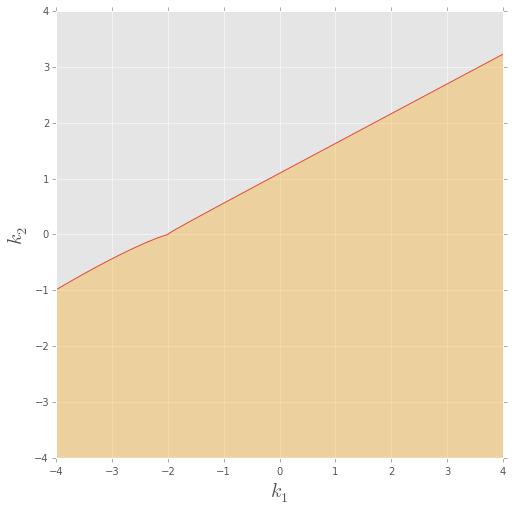
\includegraphics[width=0.5\textwidth]{../imagenes/dobintcon.png}
\caption{D-particiones de un controlador para doble integrador.}
\end{figure}

Y el sistema con este controlador será estable para los valores de
\(k_1\) y \(k_2\) escogidos tal que se encuentren en la intersección de
estas dos regiones:

\begin{figure}[htbp]
\centering
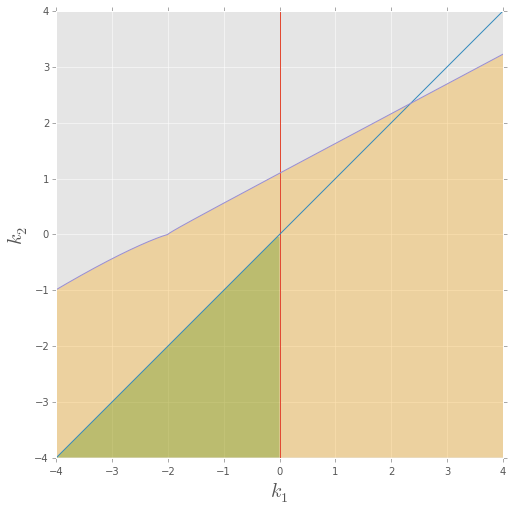
\includegraphics[width=0.5\textwidth]{../imagenes/dobint.png}
\caption{D-particiones de doble integrador.}
\end{figure}

    \subsection{Ejemplo 2 - Oscilador armónico
retardado}\label{ejemplo-2---oscilador-armuxf3nico-retardado}

    Para el sistema:

\[
\dot{x}(t) =
\begin{pmatrix}
0 & 1 \\
-1 & 0
\end{pmatrix}
x(t) +
\begin{pmatrix}
0 \\
1
\end{pmatrix}
u(t - h)
\]

con \(h = 1\).

    En lazo cerrado tiene un cuasiplolinomio:

\[
s^2 + \frac{1}{2} s\left[ -j k_1 \left( e^{jh} - e^{-jh} \right) - k_2 \left( e^{jh} + e^{-jh} \right) \right] + \frac{1}{2} \left[ -k_1 \left( e^{jh} + e^{-jh} \right) + j k_2 \left( e^{jh} - e^{-jh} \right) \right]
\]

Con una gráfica de D-particiones:

\begin{figure}[htbp]
\centering
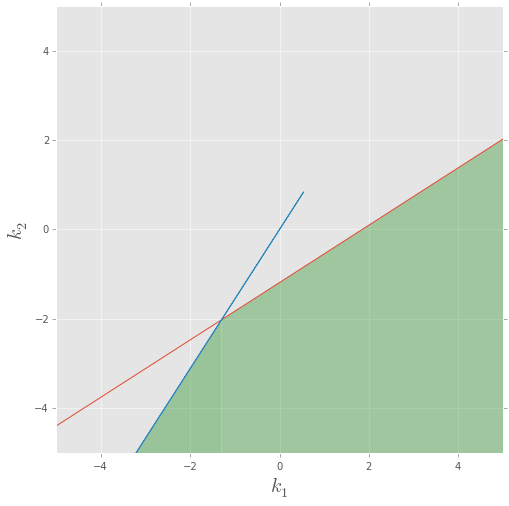
\includegraphics[width=0.5\textwidth]{../imagenes/oscarmlc.png}
\caption{D-particiones oscilador armónico retardado en lazo cerrado}
\end{figure}

    Para el controlador tenemos un cuasipolinomio caracteristico:

\[
s^2 + 1 + k_1 j \left( s \sin{(h)} - \cos{(h)} + e^{-sh} \right) + k_2 \left( \sin{(h)} + s \cos{(h)} - s e^{-sh} \right)
\]

con una gráfica de D-Particiones:

\begin{figure}[htbp]
\centering
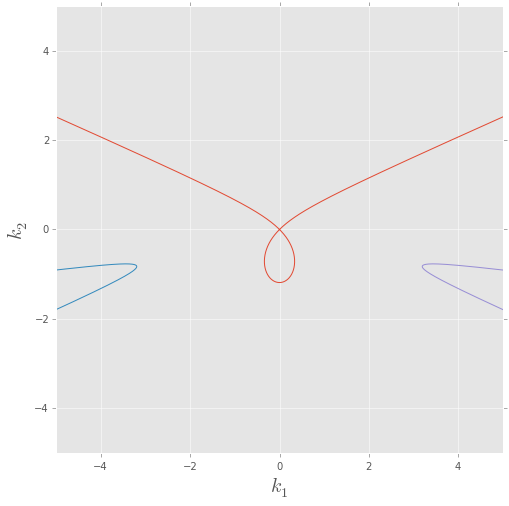
\includegraphics[width=0.5\textwidth]{../imagenes/oscarmcon.png}
\caption{D-particiones de controlador para oscilador armónico
retardado.}
\end{figure}

    \section{Implementación del método de introducción de
dinámicas}\label{implementaciuxf3n-del-muxe9todo-de-introducciuxf3n-de-dinuxe1micas}


    % Add a bibliography block to the postdoc
    
    
    
    \end{document}
